% \documentclass[margin=0mm]{standalone}
% \input{../tikz_header}


% \begin{document}





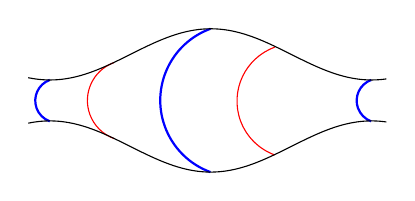
\begin{tikzpicture}[font=\footnotesize]
  %\useasboundingbox (0,0) rectangle (5,5);
  %\draw (0,0) rectangle ++(5,5);
  
  \begin{scope}[scale=1.3]
  

  \draw[thick, blue] (3.14 * 1.5, 0.2) arc [start angle=110, end angle=250, radius={0.215}] ;
  \draw[thick, blue] (3.14 * 2, 0.7) arc [start angle=110, end angle=250, radius={0.745}] ;
  \draw[thick, blue] (3.14 * 2.5, 0.2) arc [start angle=110, end angle=250, radius={0.215}] ;


  \draw[red] (3.14 * 1.7, 0.37) arc [start angle=110, end angle=250, radius={0.395}] ;
  \draw[red] (3.14 * 2.2, 0.52) arc [start angle=110, end angle=250, radius={0.56}];

  \draw[   domain=4.5:8, variable=\x,  samples=200, smooth] plot ({\x }, {0.2 + 0.5 *  cos(deg(\x))^2 ) });
  \draw[   domain=4.5:8, variable=\x,  samples=200, smooth] plot ({\x  }, {-0.2 -0.5 * cos(deg(\x))^2 )});
  \end{scope}

\end{tikzpicture}

%\end{document}